\documentclass{standalone}
\usepackage{tikz}
\usetikzlibrary{calc,patterns}
\newcommand{\footm}[1]{\mbox{\footnotesize{#1}}}
\begin{document}
	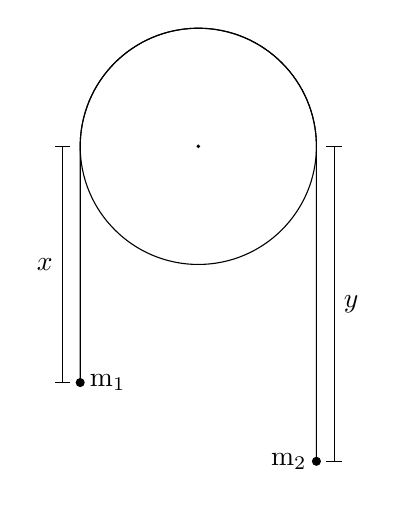
\begin{tikzpicture}
		\def\slength{3}
		\def\tlength{4}
		\def\pulleyradius{1.5}
		\def\ropethickness{.1}
		\def\gravitationalacceleration{.10}
		\def\smallmass{5}
		\def\bigmass{10}
		
		\coordinate (Pulley) at (0,0);
		\coordinate (Small) at (-\pulleyradius,-\slength);
		\coordinate (Big) at (\pulleyradius,-\tlength);
		
		\draw (Small) -- ++(0,\slength) arc[start angle = 180, end angle = 0, radius = \pulleyradius] -- ++ (0,-\tlength);
		
		\draw (Pulley) circle (\pulleyradius);
		\draw[fill] (Pulley) circle ({.01*\pulleyradius});
		
		
		\draw[fill] ({-\pulleyradius},{-\slength}) circle (.05) node[anchor = west] {\(\mbox{m}_1\)};
		\draw[fill] ({\pulleyradius},{-\tlength}) circle (.05) node[anchor = east] {\(\mbox{m}_2\)};
		
		\draw ($(Pulley) + (-1.15*\pulleyradius,0)$) --  ++ (0,-\slength) node[midway, anchor = east] (s) {\(x\)};
		\draw ($(Pulley) + (-1.15*\pulleyradius + .1,0)$) -- ++ (-.2,0);
		\draw ($(Pulley) + (-1.15*\pulleyradius + .1,-\slength)$) -- ++ (-.2,0);
		\draw ($(Pulley) + (1.15*\pulleyradius,0)$) -- ++ (0,-\tlength) node[midway, anchor = west] (t) {\(y\)};
		\draw ($(Pulley) + (1.15*\pulleyradius + .1,0)$) -- ++ (-.2,0);
		\draw ($(Pulley) + (1.15*\pulleyradius + .1,-\tlength)$) -- ++ (-.2,0);
	\end{tikzpicture}
\end{document}
